\tikzsetnextfilename{exp_origami_samples_n4}%
\begin{tikzpicture}

  \matrix[
      matrix of nodes,
      every node/.style={inner sep=0},
      column sep=1mm,
      row sep=1mm,
      ampersand replacement=\&] (samples) {
    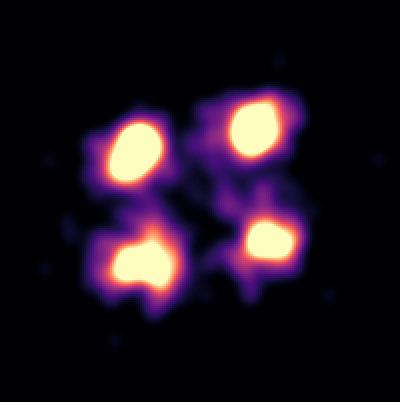
\includegraphics[width=\plotwidth]{figures/data/exp_counting/4bs_origami_1.png}
    \&
    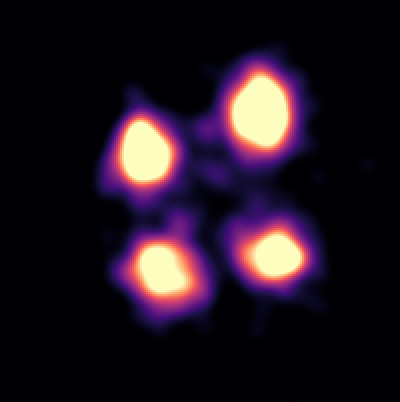
\includegraphics[width=\plotwidth]{figures/data/exp_counting/4bs_origami_2.png}
    \&
    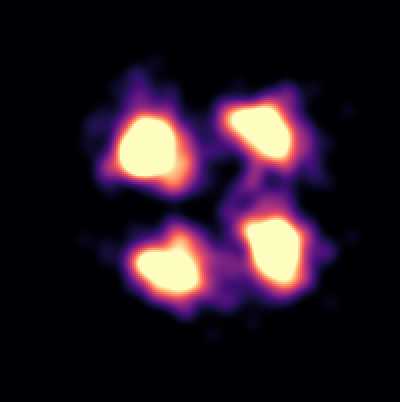
\includegraphics[width=\plotwidth]{figures/data/exp_counting/4bs_origami_3.png}
    \&
    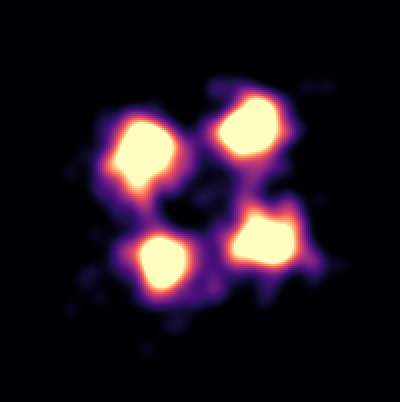
\includegraphics[width=\plotwidth]{figures/data/exp_counting/4bs_origami_4.png}
    \\
  };

  % scale bar
  \node[
    rectangle,
    minimum width=0.25\plotwidth, % images are 400px, 1/4 is 100px and that is 20nm
    fill=white,
    anchor=south east,
    inner sep=0pt,
    outer sep=2mm] (scalebar) at (samples-1-4.south east) {};
  \node[anchor=south,white] at (scalebar.center) {\tiny $20 \micrometer$};
\end{tikzpicture}
